\section{Introduction}
A long-term goal of robotics research is the introduction of
intelligent household robots.  To be effective, such robots will need
to perform complex tasks over long horizons (e.g., setting a dinner
table, doing laundry). Planning for these long-horizon tasks is
infeasible for state-of-the-art motion planners, making the need for a
hierarchical system of reasoning apparent.

One way to approach hierarchical planning is through combined
\emph{task and motion planning} (TAMP). In this approach, an agent is
given a symbolic, logical characterization of actions (e.g., move,
grasp, putdown), along with a geometric encoding of the
environment. TAMP systems maintain a hierarchical separation of
high-level, symbolic task planning and low-level, geometric motion
planning.  Efficient integration of these two types of reasoning is
difficult, and recent research has proposed several methods for
it~\cite{srivastava2014combined, kaelbling2011hierarchical,
  lagriffoul2014orientation, GarrettWAFR14, dornhege2012semantic}.
We adopt the principles of abstraction in the TAMP system developed by
Srivastava et al.~\cite{srivastava2014combined} (henceforth referred
to as SFRCRA-14) to factor the reasoning and search problems into
interacting logic-based and geometric components.

\begin{figure}[t]
  \centering
    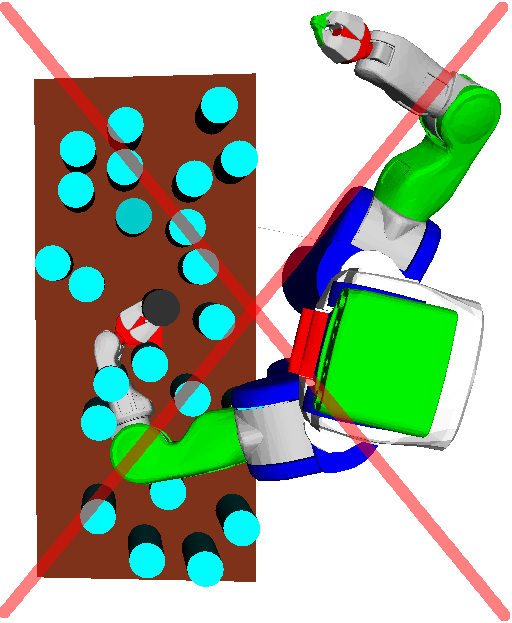
\includegraphics[scale=0.17]{images/grasp_teaser_bad.png}
    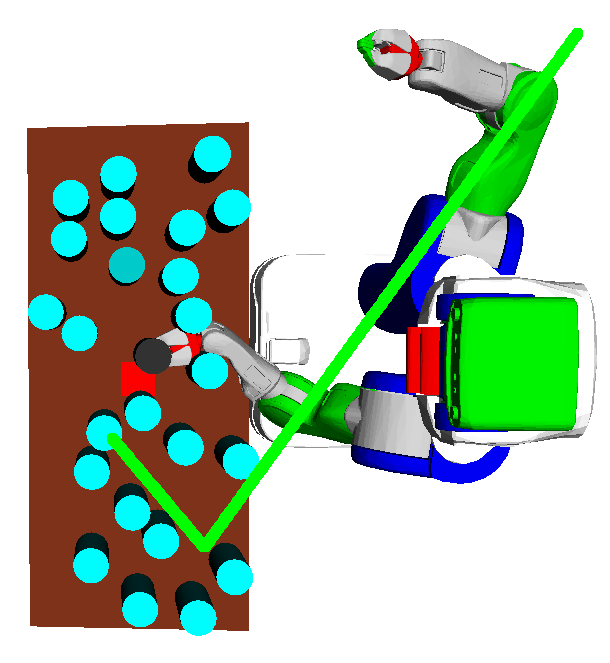
\includegraphics[scale=0.17]{images/grasp_teaser_good.png}
  \caption{\small{When trying to grasp the black can, the grasping pose sampled by a robot can
significantly affect the quality of the obstructions determined. In the left image, 6 objects (shown in red) obstruct the
grasping trajectory, but in the right one, only 2 do. The new plan proposed from the right image thus only
requires moving 2 obstructions out of the way. In this work, we integrate machine learning into our task and
motion planning system using expert demonstrations, to learn an ordering on plan exploration. The system
learns to prefer simpler and more feasible plans, such as the one resulting from the scenario on the right.}}
  \label{fig:cover}
\end{figure}

Recent work~\cite{chitnis2015mlpc} that builds on SFRCRA-14 proposes
methods for jointly carrying out guided search in the space of
high-level (logic-based) plans and their low-level
\emph{refinements}, instantiations of continuous values for
symbolic references in the plan. We refer to this search for a valid low-level
refinement as \emph{plan refinement}. In this paper, we improve upon
the recent work's preliminary methods for high-level search, while retaining its methods
for learning low-level refinement distributions.

As in Chitnis et al.~\cite{chitnis2015mlpc}, we make use of unpublished work
recently submitted for review to ICRA 2016. The work develops
a \emph{plan refinement graph}, a data structure that stores a
set of qualitatively different high-level plans that could solve a task (the graph is
described in detail in Section IV-B).
During planning, we repeatedly select one such plan and either 1) try to
refine it or 2) incorporate geometric information in order to generate a new high-level
plan. This allows interleaving plan refinement with a
search over \emph{which} high-level plan to try refining, given options
that address different infeasibilities.

We present machine learning techniques used in learning from demonstrations
to train heuristic functions that guide the search process over the high level.
This amounts to learning to predict how difficult it is to refine a given plan.
Many TAMP systems rely on hand-coded heuristics to achieve this. We develop a system that uses human
demonstrations of optimal plan-space trajectories to learn intelligent navigation
of the plan refinement graph. We use 1) a max-margin formulation, which is commonly used in inverse reinforcement learning, along with Dataset Aggregation (DAgger)~\cite{ross2010dagger} and 2) a discriminative formulation using logistic regression.

The contributions of our work are as follows: 1) we formulate navigation through a plan
refinement graph as an MDP; 2) we present a method that trains
heuristics for intelligently searching the available space of task plans, through learning
from expert demonstrations; and 3)
we run experiments to evaluate the performance of our system in a
variety of simulated domains. We show improvements in performance over both SFRCRA-14
and the preliminary system developed by Chitnis et al.~\cite{chitnis2015mlpc}.
